% !TeX spellcheck = en_EN-English

\section{Embedding of patient}
\label{embeddingRes}

First of sub-tasks for prediction of patient future costs is to embed each patient record into numerical vector that would be understandable for neural network. For each record of a patient we embed four information. First and easy to implement is a timestamp which is computed using numerical and date values, then there three more tricky information and those are diagnosis, medical procedure and prescribed drug. 


\subsection{Diagnosis embedding}

We need to confirm that closely related diagnosis would get embedding with smaller distance meaning higher similarity compared to less related diagnosis.
In order to confirm that our embedding has desired properties we computed similarity of embedding of multiple codes. As similarity function we choose simple multiplicative inverse of Euclidean distance. In Tab. \ref{tab:diag_emb_show} we can see results. Highest similarity was between codes G47.30 and G40.09 which is expected since they belong to same main category and very close subcategory, second highest was between H40.09 and H18.80 which are only other combination that belong to same main category, this confirms that main category has biggest impact since this similarity is significantly higher than that between G40.09 and H40.09 which differ only main category.

\begin{table}[!h]
	\centering
	\begin{tabular}{|l|l|l|}
		\hline
		Code A & Code B & Similarity \\ \hline
		G47.30 & G40.09 & 2.77       \\ \hline
		G47.30 & H40.09 & 0.53       \\ \hline
		G47.30 & H18.80 & 0.46       \\ \hline
		G40.09 & H40.09 & 0.54       \\ \hline
		G40.09 & H18.80 & 0.45       \\ \hline
		H40.09 & H18.80 & 0.84       \\ \hline
	\end{tabular}
	\caption{Similarities of embedding of multiple chosen MKCH-10 codes}
	\label{tab:diag_emb_show}
\end{table}  

Another confirmation that embeddings works as intended by clustering them. More specifically we would expect that if we group embeddings into as many clusters as are main categories, each cluster should contain mostly if not only diagnosis from one main category. On order to test this we used K-means clustering with 26 clusters which is number of different main categories of diagnosis and got these results:

\begin{table}[!h]
	\centering
	\begin{tabular}{|p{0.15\textwidth}|p{0.2\textwidth}|p{0.5\textwidth}|}
		\hline
		Cluster ID & Cluster size & Frequency of first level values \\ \hline
		0 & 654 & C: 654, \\ \hline
		1 & 2092 & M: 2092, \\ \hline
		2 & 766 & Y: 766, \\ \hline
		3 & 543 & S: 543, \\ \hline
		4 & 786 & Z: 786, \\ \hline
		5 & 1100 & T: 1100, \\ \hline
		6 & 1067 & X: 1067, \\ \hline
		7 & 620 & H: 496, U: 124, \\ \hline
		8 & 752 & S: 752, \\ \hline
		9 & 1770 & M: 1770, \\ \hline
		10 & 739 & Q: 739, \\ \hline
		11 & 584 & D: 584, \\ \hline
		12 & 507 & F: 507, \\ \hline
		13 & 958 & W: 958, \\ \hline
		14 & 556 & E: 556, \\ \hline
		15 & 491 & A: 491, \\ \hline
		16 & 553 & O: 553, \\ \hline
		17 & 627 & K: 627, \\ \hline
		18 & 872 & V: 872, \\ \hline
		19 & 521 & G: 521, \\ \hline
		20 & 463 & L: 463, \\ \hline
		21 & 420 & R: 420, \\ \hline
		22 & 465 & B: 465, \\ \hline
		23 & 717 & J: 319, P: 398, \\ \hline
		24 & 568 & I: 568, \\ \hline
		25 & 535 & N: 535, \\ \hline
	\end{tabular}
	\caption{Size of clusters and frequencies of first level diagnosis codes in them.}
	\label{tab:diag_clusters}
\end{table}

In Tab. \ref{tab:diag_clusters} we can see that almost every cluster consist of diagnosis from with only single main category. Only immediately visible issues are clusters 7 and 23 where two main categories got assigned same cluster which is most likely caused by their small size compared to other and by the fact that largest categories M and S got split into two clusters.

\subsection{Drug embedding}

To confirm this we do similar check as we did with diagnosis code and compute similarity of four chosen ATC codes and see if our theory holds. To compute similarity we again use multiplicative inverse of Euclidean distance. We choose C01EB15, C01CA04, C10AA07 and J01CA04, we would expect first two to be most similar since they match on first levels, than first two compared to third should have slightly lower similarity since they match on only first level and finally we expect that all three would be least similar to fourth one since first level is different, even though that second and forth match on all other levels.  We can see results in Tab. \ref{tab:drug_emb_show}. We can see that results met our expectation with highest similarity between first two and lowest between any of first three and fourth, even in case of second and forth that match on all other levels except first.

\begin{table}[!h]
	\centering
	\begin{tabular}{|l|l|l|}
		\hline
		Code A & Code B & Similarity \\ \hline
		C01EB15 & C01CA04 & 1.24      \\ \hline
		C01EB15 & C10AA07 & 0.54       \\ \hline
		C01EB15 & J01CA04 & 0.45       \\ \hline
		C01CA04 & C10AA07 & 0.64       \\ \hline
		C01CA04 & J01CA04 & 0.48       \\ \hline
		C10AA07 & J01CA04 & 0.38       \\ \hline
	\end{tabular}
	\caption{Similarities of embedding of multiple chosen ATC codes}
	\label{tab:drug_emb_show}
\end{table}  

Also similarly to diagnosis we can test whether our embeddings would cluster mainly first level of code or not. Since there are 14 main anatomical or pharmacological groups as shown on Fig. \ref{fig:atc_l1} we used K-means algorithm with 14 clusters and got these results:
\\

\begin{table}[!h]
	\centering
	\begin{tabular}{|p{0.15\textwidth}|p{0.2\textwidth}|p{0.5\textwidth}|}
		\hline
		Cluster ID & Cluster size & Frequency of first level values \\ \hline
		0 & 8645 & C: 8645, \\ \hline
		1 & 19132 & N: 19132, \\ \hline
		2 & 9322 & L: 8657, S: 665, \\ \hline
		3 & 11734 & A: 11734, \\ \hline
		4 & 7159 & B: 7159, \\ \hline
		5 & 9526 & V: 9526, \\ \hline
		6 & 4681 & R: 4681, \\ \hline
		7 & 14732 & C: 14732, \\ \hline
		8 & 7237 & V: 7237, \\ \hline
		9 & 4031 & M: 3987, P: 44, \\ \hline
		10 & 3599 & G: 3599, \\ \hline
		11 & 2367 & N: 2367, \\ \hline
		12 & 9032 & D: 1266, G: 897, H: 1136, J: 5733, \\ \hline
		13 & 6093 & N: 6075, P: 18, \\ \hline
	\end{tabular}
\caption{Size of clusters and frequencies of first level drug codes in them.}
\label{tab:drug_clusters}
\end{table}

Based on results we can see on Tab. \ref{tab:drug_clusters} we concluded that embeddings works generally as intended. We can see that clusters mostly consist of embeddings with same first level values. There are some exceptions which are most likely caused by uneven number of drug in each category. Because of this categories with smallest number of drug like P, S, D, H or G got assigned to cluster along with bigger category and categories with biggest number of drugs like N, C or V got split into multiple categories.  
\\

Based on results of these tests we can conclude that embeddings works generally as intended.

\subsection{Medical procedure embedding}

As said in previous chapters we tried two different approaches both using pretrained models. After we embed medical procedure descriptions both ways we quickly found out that a lot of procedures did not received any embedding from Word2vec model, more specifically 731 out of 7329 procedures, so almost 10\% were not embedded, and even among procedures that receive any kind of embedding there were a lot words that were not embedded and so they didn't contributed to resulting embedding. This was caused mostly by limitations of Word2vec model that is able to embed only words which are in it's dictionary, so words available in it's training corpus, and it seems like a lot of professional medical terms such as 'polycystické' or 'cytokín' were not in corpus. Similar issue potentially could have happened also while using LaBSE model, however we found no case where LaBSE model was not able whole procedure. Also thanks to most professional medical terms being similar across multiple languages and fact that LaBSE model was trained on much bigger corpus consisting of 109 distinct languages it's highly probable that much more terms were successfully embed creating much better embedding of whole description. 
\\

Since results of embedding using Word2vec model has a lot of issue we decided to proceed using only LaBSE model which was at least able to embed all descriptions. This model gave us embedding with 768 dimensions, in order to densify this information while maintaining most of it we decided to use PCA. We specifically wanted to first few dimensions that would explain over 90\% of variance, since in the case of PCA, the fraction of explained variance is often used as a good proxy for the fraction of preserved information. After running this algorithm we ended up with 119 dimensional embedding that explained 90.4\% of variance of original embedding.
\\

To confirm that resulting embedding successfully encode description of procedure and gave similar procedures similar embedding we did same thing as in case of drug and disease embedding validation and try to group embeddings using K-means algorithm. However in this case we did not have any information similar to highest level of codes for drugs and diagnosis on which we could base our validation, so we decided to just manually look through clusters to assess whether procedures inside them have meaningful connections.
\\

Since we have 7329 procedures we choose our K, so number of clusters, to be 365 to have on average close to 20 procedures in single group. This decision was mostly arbitrary. After checking multiple clusters we found cases such as group cluster number 215 which procedures are listed in Fig. \ref{fig:G215} where we can see that all procedures has something to do with transplantation. However in some cases clusters contained mixture of seemingly random procedures, such as procedures in cluster 45 in Fig. \ref{fig:G45} where we can see mixture evaluation of final reports mixed with investigation of pharmacokinetics and papillosphincterotomy, fortunately it seems content of clusters like these is not purely random but consist of multiple subgroups which might indicate embedding works as intended and we just clustered procedures into too few groups.


\begin{figure}[!h]
	\centering
	
	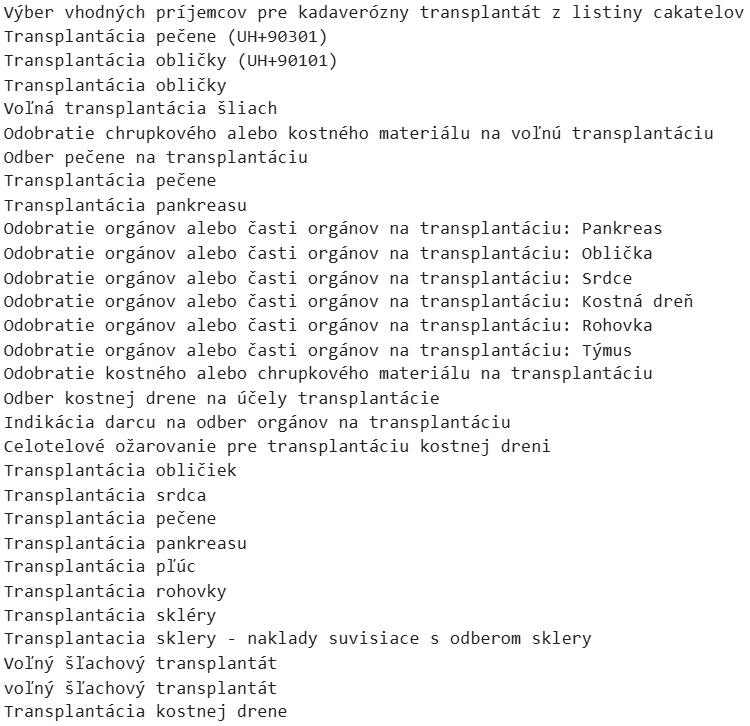
\includegraphics[width=0.6\textwidth]{images/G215.png}
	
	\caption{Medical procedures grouped in cluster number 215.}
	\label{fig:G215}
\end{figure}

\begin{figure}[!h]
	\centering
	
	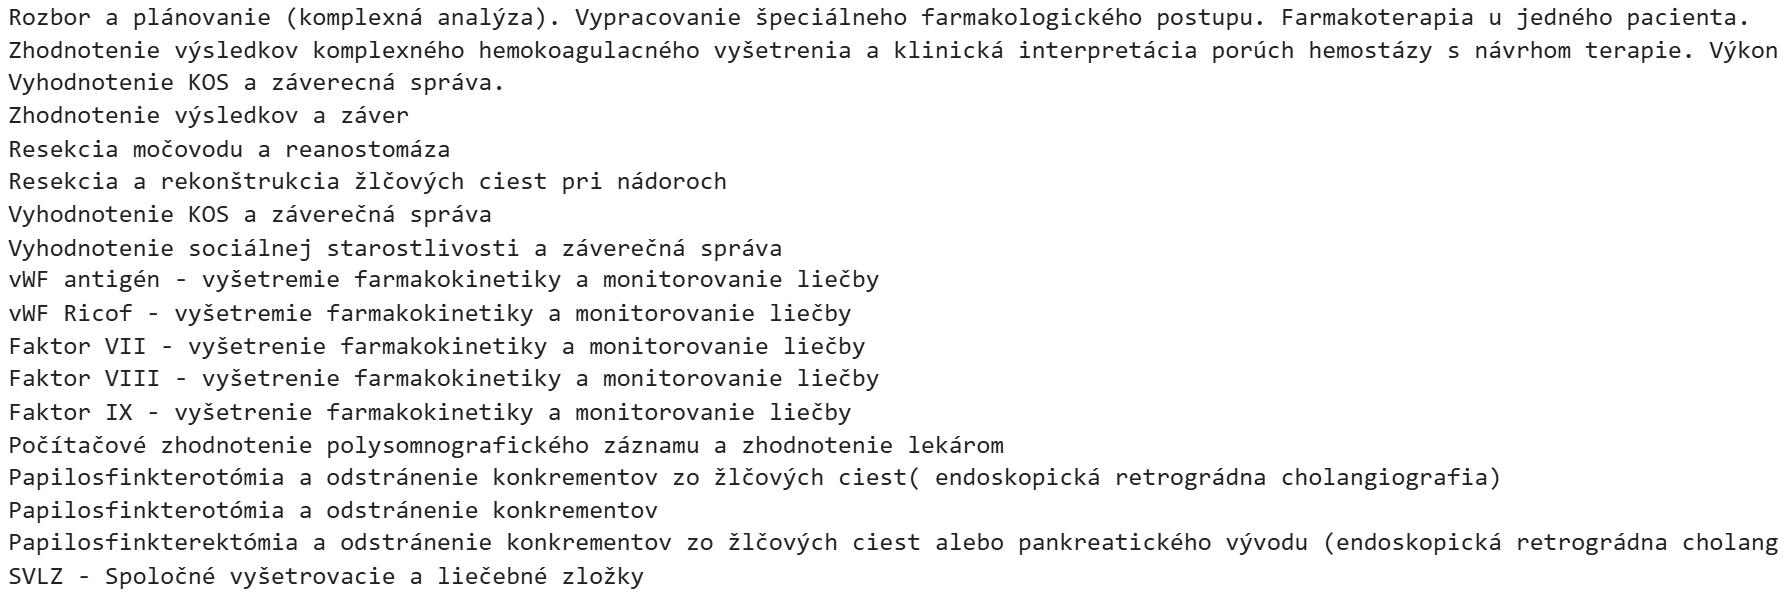
\includegraphics[width=1.1\textwidth]{images/G45.png}
	
	\caption{Medical procedures grouped in cluster number 45.}
	\label{fig:G45}
\end{figure}